%! alt Triangle ABC with AB = 13, BC = 14 and CA = 15, and its inscribed circle with centre I. The radius r from I meets BC at right angles at the touch point D. Segments from I to the three vertices split the triangle into three smaller triangles whose heights are all r.
%! after_paragraph 1
%! scale 1/2
% The shared preamble of every Kyuclid figure. pipeline/figures turns these colours into theme-aware paint,
% and refuses any other colour, so draw only with them:
%   figink (lines and labels), figaux (construction lines), figaccent (the object the argument turns on),
%   figtint and figaccenttint (light fills).
\documentclass[border=1.5pt]{standalone}
\usepackage{tkz-euclide}
\definecolor{figink}{RGB}{0,0,0}
\definecolor{figaux}{RGB}{85,85,85}
\definecolor{figaccent}{RGB}{192,57,43}
\definecolor{figtint}{RGB}{221,221,221}
\definecolor{figaccenttint}{RGB}{245,213,208}
% tkz-euclide's defaults draw circles, compasses and marks in 50% grey and fill points with a tint.
\makeatletter
\def\tkz@otherlinecolor{figink}
\def\tkz@euc@circlecolor{figink}
\def\tkz@euc@compasscolor{figink}
\def\tkz@euc@mkcolor{figink}
\def\tkz@mk@fill{figink}
\def\tkz@euc@pointfillcolor{figink}
\makeatother
\tkzSetUpLine[color=figink,line width=.7pt]
\tkzSetUpArc[color=figink,line width=.7pt]
\tkzSetUpCompass[color=figink,line width=.5pt]
\tkzSetUpPoint[color=figink,fill=figink,size=3.1pt]
\tikzset{
  every picture/.style={line cap=round,line join=round,color=figink},
  circle style/.append style={color=figink,line width=.7pt},
  aux/.style={color=figaux,line width=.45pt,dash pattern=on 2.6pt off 2pt},
  key/.style={color=figaccent,line width=1pt},
  mk/.style={color=figink,line width=.5pt},
  lbl/.style={color=figink,inner sep=2.2pt},
  len/.style={color=figink,inner sep=1.5pt,font=\small},
}

\begin{document}
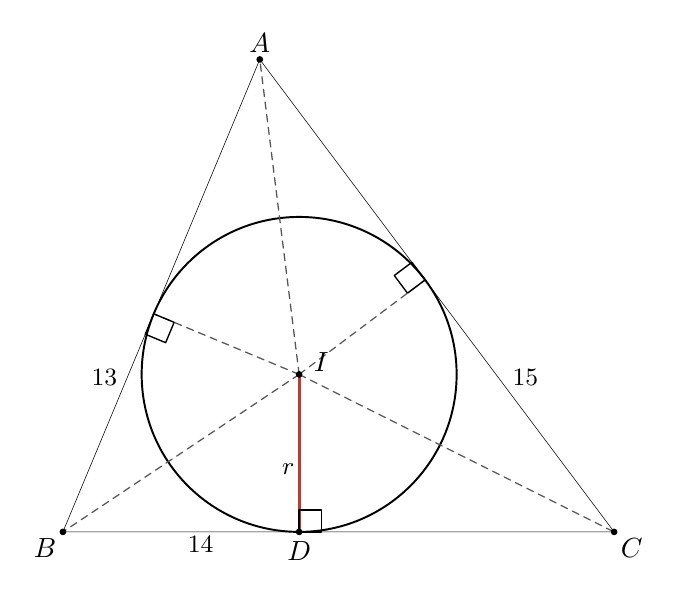
\begin{tikzpicture}
\tkzDefPoint(0.0,0.0){B} %! B = (0, 0)
\tkzDefPoint(7.0000000,0.0){C} %! C = (14, 0)
\tkzDefPoint(2.5000000,6.0000000){A} %! A = (5, 12)
\tkzDefPoint(3.0000000,2.0000000){I} %! I = incentre(A, B, C)
\tkzDefPoint(3.0000000,0.0){D} %! D = foot(I, B, C)
\tkzDefPoint(4.6000000,3.2000000){E} %! E = foot(I, C, A)
\tkzDefPoint(1.1538462,2.7692308){F} %! F = foot(I, A, B)
%! fact dist(A, B) == 13
%! fact dist(B, C) == 14
%! fact dist(C, A) == 15
%! fact area(A, B, C) == 84
%! fact tangent(I, 4, B, C)
%! fact tangent(I, 4, C, A)
%! fact tangent(I, 4, A, B)
%! fact dist(I, D) == 4
\tkzDrawCircle(I,D)
\tkzDrawSegments[aux](I,A I,B I,C)
\tkzDrawSegments[aux](I,E I,F)
\tkzDrawPolygon(A,B,C)
\tkzDrawSegment[key](I,D)
\tkzMarkRightAngle[size=.28,mk](I,D,C)
\tkzMarkRightAngle[size=.28,mk](I,E,A)
\tkzMarkRightAngle[size=.28,mk](I,F,B)
\tkzDrawPoints(A,B,C,I,D)
\tkzLabelPoint[above,lbl](A){$A$}
\tkzLabelPoint[below left,lbl](B){$B$}
\tkzLabelPoint[below right,lbl](C){$C$}
\tkzLabelPoint[right=3pt,yshift=4.5pt,lbl](I){$I$}
\tkzLabelPoint[below=1pt,lbl](D){$D$}
\tkzLabelSegment[left,pos=.6,len](I,D){$r$}
\tkzLabelSegment[above left,pos=.3,len](B,A){$13$}
\tkzLabelSegment[below,pos=.25,len](B,C){$14$}
\tkzLabelSegment[above right,pos=.3,len](C,A){$15$}
\end{tikzpicture}
\end{document}
